\documentclass[12pt,crop,tikz]{standalone}

\providecommand{\rootdir}{..}
\usetikzlibrary{automata, arrows, calc, positioning}

\tikzstyle{arrow} = [thick,->,>=stealth]

% The Tableau20 colours
\definecolor{TabLightOrange}{RGB}{255,187,120}
\definecolor{TabOrange}{RGB}{255,127,14}
\definecolor{TabLightBlue}{RGB}{174,199,232}
\definecolor{TabBlue}{RGB}{31,119,180}
\definecolor{TabGreen}{RGB}{44,160,44}
\definecolor{TabLightGreen}{RGB}{152,223,138}
\definecolor{TabSalmon}{RGB}{255,152,150}
\definecolor{TabRed}{RGB}{214,39,40}
\definecolor{TabPurple}{RGB}{148,103,189}
\definecolor{TabLightPurple}{RGB}{197,176,213}
\definecolor{TabLightPink}{RGB}{247,182,210}
\definecolor{TabPink}{RGB}{227,119,194}
\definecolor{TabLightBrown}{RGB}{196,156,148}
\definecolor{TabBrown}{RGB}{140,86,75}
\definecolor{TabGray}{RGB}{127,127,127}
\definecolor{TabOlive}{RGB}{188,189,34}
\definecolor{TabLightOlive}{RGB}{219,219,141}
\definecolor{TabLightGray}{RGB}{199,199,199}
\definecolor{TabLightCyan}{RGB}{158,218,229}
\definecolor{TabCyan}{RGB}{23,190,207}

\begin{document}
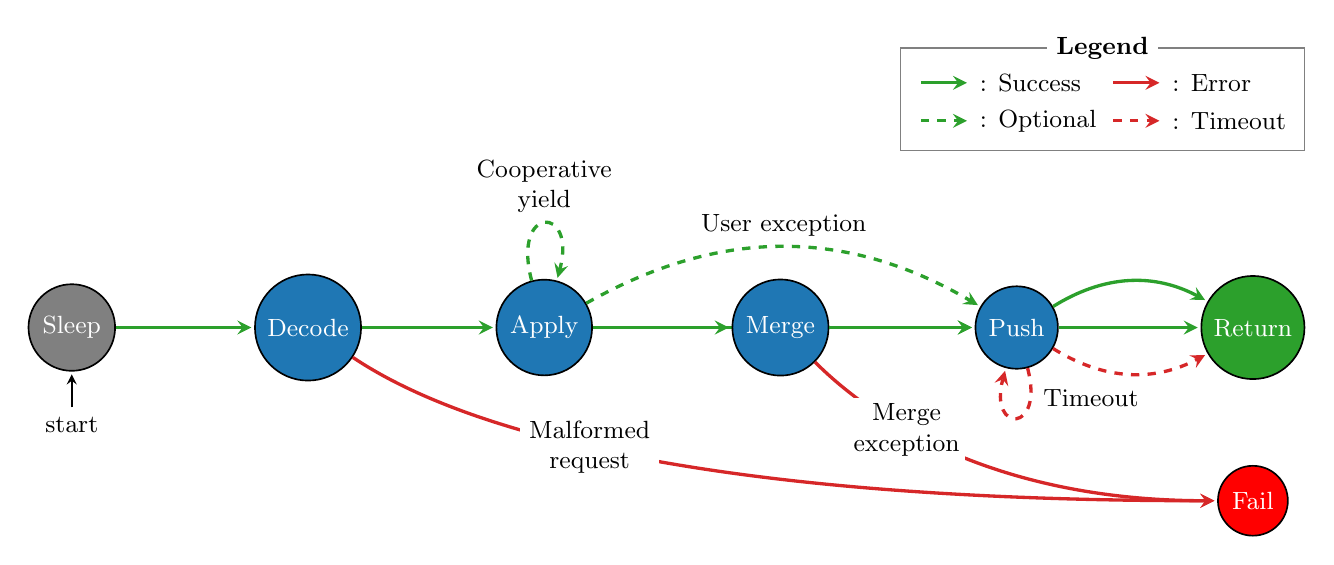
\begin{tikzpicture}
  [ every node/.style={font=\small}
  , every state/.style={fill=TabBlue,draw=black,text=white}
  , sleep/.style={fill=gray}
  , lbl/.style={align=center}
  , slbl/.style={lbl, very thick, draw=TabGreen}
  , olbl/.style={lbl, very thick, dashed, draw=TabGreen}
  , tlbl/.style={lbl, very thick, dashed, draw=TabRed}
  , err/.style={lbl, very thick, draw=TabRed}
  , ->
  , >=stealth
  , shorten >=1pt
  , node distance=3cm
  , semithick
  , on grid
  ]
  
  \node[initial, initial where=below, state,sleep] (sleep) {Sleep};
  \node[state] (decode) [right of=sleep] {Decode};
  \node[state] (apply) [right of=decode] {Apply};
  \coordinate[right=of apply] (merge);
  \node[state] (push) [right of=merge] {Push};
  \node[state,sleep,fill=TabGreen,text=white] (return) [right of=push] {Return};
  \node[state,sleep, fill=red,text=white] (fail) [below = 2.2cm of return] {Fail};

  \path (sleep) edge[slbl] node[lbl, auto, font=\footnotesize\ttfamily] {} (decode)
  (decode) edge[slbl] node {} (apply)
  (apply) edge[olbl, bend left] node[lbl, above] {User exception} (push);


  \onslide<1-2>{\path (apply) edge[slbl] node {} (push);}

  \onslide<1-3>{
    \path (push) edge [tlbl, dashed, loop below] node[above right, xshift=0.2cm] {Timeout} (push);
    \path (push) edge[slbl] node[above left] {} (return);
  }
  
  \onslide<4->{
    \path (push) edge[tlbl, bend right] node[below right] {} (return);
    \path (push) edge[slbl, bend left] node[above left] {} (return);
  }
  
  \onslide<2->{
    \path (apply) edge [olbl, dashed, loop above] node {Cooperative\\ yield} (apply);
  }
  
  \onslide<3->{
    \node[state] (merge) [right of=apply] {Merge};
    \path (apply) edge[slbl] node {} (merge)
    (merge) edge[slbl] node {} (push);
    \draw[err] (merge) .. controls +(1, -1) and +(-3.5, 0) .. (fail) node[pos=0.4, lbl, outer sep = 0pt, inner sep = 2pt, fill=white] {Merge \\ exception};
  }
  
  
  \draw[err] (decode) .. controls +(1.5,-1) and +(-8, 0) .. (fail) node[pos=0.5, lbl, fill=white] {Malformed\\ request};

  \begin{scope}[local bounding box = legend]
  \matrix [above right] at ($ (current bounding box.north east) + (-5.0, 0.0) $) {
    \node [rectangle, minimum width = 6mm, label=right:{: Success}] (legend-arrow) {}; &
    \node [rectangle, minimum width = 6mm, label=right:{: Error}] (error-arrow) {}; \\
    \node [rectangle, minimum width = 6mm, label=right:{: Optional\ \ }] (optional-arrow) {}; &
    \node [rectangle, minimum width = 6mm, label=right:{: Timeout}] (timeout-arrow) {}; \\
  };
\end{scope}

  \def\titlepad{0.1}
  \coordinate (legend-nw) at ($ (legend.north west) + (-0.15, \titlepad)$);
  \coordinate (legend-ne) at ($ (legend.north east) + (0, \titlepad) $);
  \coordinate (legend-sw) at ($ (legend.south west) + (-0.15, 0) $);
  \coordinate (legend-se) at ($ (legend.south east) $);
  \draw[gray] (legend-nw) rectangle (legend-se);

  \node[rectangle, fill=white] at ($(legend-nw)!0.5!(legend-ne)$) (legend_label) {\textbf{Legend}};

  \draw[->, slbl] (legend-arrow.west) -- (legend-arrow.east);
  \draw[->, err] (error-arrow.west) -- (error-arrow.east);
  \draw[->, tlbl] (timeout-arrow.west) -- (timeout-arrow.east);
  \draw[->, olbl] (optional-arrow.west) -- (optional-arrow.east);
\end{tikzpicture}
\end{document}